% 统计力学玻尔兹曼分布

\section{统计力学玻尔兹曼分布}
\subsubsection{体系的微观状态}
粒子的一个微观状态在\(\mu \)空间中对应一点,
一个体系的微观状态对应\(N\)个点,
粒子的微观状态随时间的变化对应一根线。
体系的微观状态随时间的变化对应\(N\)根线。
某个粒子的微观状态随时间变化的这根线不相交(与牛顿方程的单值性违背(保守力学体系))。

\subsection{相格}
引入相格。相格需
\begin{itemize}
  \item 足够大: 可含足够多代表点
  \item 足够小:一个相格内不同点的\(\{\vb{q}, \vb{p}\}\)看作近似相等
\end{itemize}
给相格进行编号,给粒子进行编号。
\begin{definition}[配容]
每个相格中既问有几点,又问哪几点的分配方式。
\end{definition}
同相格内部代表点交换,微观态不变,配容不变;
不同相格内部代表点交换,微观态变,配容变。

\subsection{体系的宏观状态}
每个相格中问有几点,不问哪几点。

一个宏观态对应多少微观态?
在不同相格交换的次数\({N!} / {\prod_l a_l!}\)。
\\ 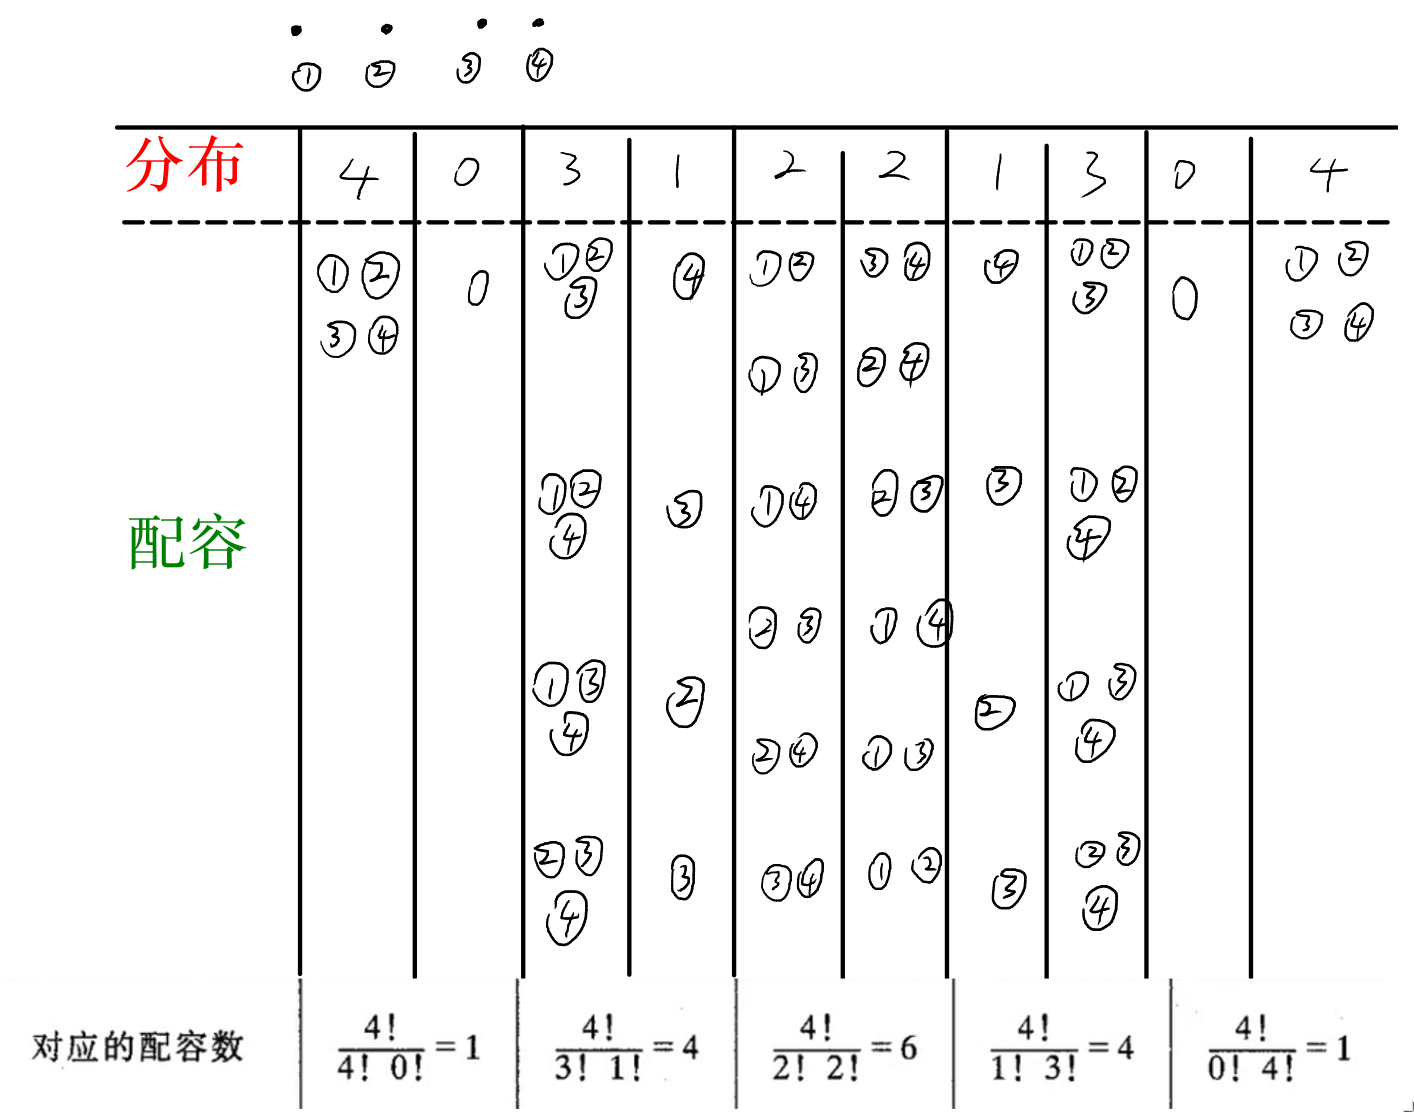
\includegraphics[width=0.8\textwidth]{figures/2022-09-07T220102+0800.png} \\

\subsection{体系的平衡态,最概然分布}
\begin{definition}[进入第\(l\)个相格的概率]
  \begin{equation}
    g_l = \frac{\Delta \omega_l}{\omega}
  \end{equation}
\end{definition}

基本假定:
\begin{enumerate}
  \item 先验\sn{不加约束条件}机率相等\sn{每个代表点进到相格的机率与相格的大小成比例}:\(g_i = g_j = \dots\)
  \item 平衡态是最可几\sn{出现机率最大}的宏观态
\end{enumerate}
\begin{margintable}
  \begin{description}
  \item[\(\Delta \omega_l\)]   第\(l\)个相格的体积  \\
  \item[\(g_l\)]   撒一颗豆子落到第\(l\)个相格的概率  \\
  \item[\(g_l^{a_l}\)]   撒N个豆子,有\(a_l\)颗落到第\(l\)个相格的概率
  \end{description}
\end{margintable}
\begin{marginfigure}
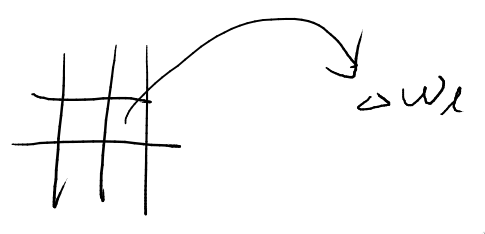
\includegraphics[width=\textwidth]{figures/2022-09-07T223529+0800.png} \\
\end{marginfigure}
对于某个宏观态,第$l$个相格有\(a_l\)个点,\(l \in [1, L]\),\(L\)为相格总数,则每个微观观态出现的概率都为
\begin{equation*}
  \underbrace{g_1 g_1 g_1\dots}_{a_1\text{个}}
  \underbrace{g_2 g_2 g_2\dots}_{a_2\text{个}}
  \underbrace{g_l g_l g_l\dots}_{a_l\text{个}}
  = \prod_l g_l^{a_l}
\end{equation*}
该宏观态有\({N!} / (\prod_l a_l !)\)个微观态,那么这个宏观态出现的概率为
\begin{equation}
  \begin{aligned}
  W 
  &=\underbrace{\left(\prod_l g_l^{a_l}+\prod_l g_l^{a_l}+\prod_l g_l^{a_l}+\dots\right)}_{\frac{N!}{\prod_l a_l!} \text{个微观态}} \\
  &= \frac{N!}{\prod_l a_l!} \prod_l g_l^{a_l}=
\frac{N!}{\prod_l a_l!}
\prod_l \left(\frac{\Delta \omega_l}{\omega}\right)^{a_l}\\
    &=
\left(\prod_l \frac{1}{\omega^{a_l}}\right)
\cdot
\left(\frac{N!}{\prod_l a_l!}
\prod_l {\Delta \omega_l}^{a_l}
\right) \\
    &=
\left(\frac{1}{\omega}\right)^{\sum_l a_l}
\cdot
\left(\frac{N!}{\prod_l a_l!}
\prod_l {\Delta \omega_l}^{a_l}
\right) \\
  \end{aligned}
\end{equation}
又因为每个微观态出现的先验机率相等
\begin{equation}
\prod_l g_l^{a_l}=\left(\frac{\Delta \omega_l}{\omega}\right)^{a_l}
=\left(\frac{\Delta \omega}{\omega}\right)^{a_l}
\end{equation}




%%% vim: set ts=2 sts=2 sw=2 isk+=\: et cc=+1 formatoptions+=mM:
